% Generated by Scripts/build-release-documents.py from release Markdown.
\documentclass[11pt,letterpaper]{article}
\usepackage[margin=1in]{geometry}
\usepackage[T1]{fontenc}
\usepackage{tgpagella}
\pdfinterwordspaceon
\usepackage{enumitem}
\setlist[itemize]{leftmargin=*,itemsep=.1em}
\usepackage{pdfpages}
\usepackage[colorlinks=true,urlcolor=blue,linkcolor=blue]{hyperref}
\hypersetup{pdftitle={TeXShop Changes},pdfauthor={TeXShop contributors}}
\setcounter{secnumdepth}{0}
\setlength{\parindent}{0pt}
\setlength{\parskip}{.3em}
\setlength{\emergencystretch}{2em}
\begin{document}
\section{TeXShop 5.60}

\noindent\textit{Release preparation; not yet published.}\par

TeXShop 5.60 fixes typesetting cancellation and keeps the PDF preview position on macOS 27. It adds LaTeX-aware spell checking, pinnable and movable link previews, a redesigned Settings window with automatic detection of TeX and Ghostscript, Command-0 for the console, and a new app icon.


\subsection{Typesetting and stability}

\begin{itemize}
\item \textbf{Critical fix:} Fix a problem where Stop reported that typesetting had been aborted but left TeX running. Starting another typesetting job now also stops the previous job and its child processes.
\item Run Experiment jobs in a separate console with independent input, cancellation and cleanup, so they do not interfere with normal typesetting. Closing or replacing an Experiment cancels only its own job. Reported by \href{https://github.com/Uwe-Schmock}{Uwe Schmock} (\href{https://github.com/TeXShopProject/TeXShop/issues/8}{\#8}).
\item Handle failures to launch typesetting tools and missing command-search paths more reliably, and avoid an indefinite wait when stopping helper processes.
\item Show a sheet when a specified TeX root file cannot be found.
\item Fix errors involving empty documents, isolated quotation marks, and save-completion handling.
\item Improve the handling of console output and log files that contain mixed encodings or broken characters, including UTF-8 characters split by TeX’s line wrapping.
\end{itemize}

\subsection{LaTeX-aware spell checking}

\begin{itemize}
\item Add LaTeX-aware spell checking, based on suggestions from \href{https://github.com/ralphrmartin}{Ralph Martin}. It checks prose while skipping TeX commands, comments, mathematics, and arguments used for references and similar purposes. The feature is enabled by default and can be turned off under Settings \(\rightarrow\) Spell Checking.
\item Recognize supported macro definitions and language-switching commands when identifying text to check. The spelling panel can check passages in the specified language.
\item Add editable spelling-exclusion rules, a replacement field and Change All for words in the checked text, and a way to forget learned words found in the current document. A Change All operation can be undone in one step.
\item Fill the replacement field for Change All with the suggestion selected in the spelling panel, by clicking it or with the arrow keys. When there is only one suggestion, it is filled in as soon as the word is shown. The text changes only when Change All is used. Proposed by \href{https://github.com/ralphrmartin}{Ralph Martin}.
\item Make Change in the spelling panel beep and do nothing, as Change All does, when other text has been selected or the document edited since the word was shown, instead of replacing that text. Proposed by \href{https://github.com/ralphrmartin}{Ralph Martin}.
\item Improve Find Next, scrolling to misspelled words, and spell-checking performance in long documents and split editors.
\end{itemize}

\subsection{External file changes and PDF preview}

\begin{itemize}
\item Use the recorded source-click position and the clicked split editor for SyncTeX, including clicks at the start of a line and context-menu actions. Match valid filesystem aliases to SyncTeX inputs, prefer an exact recorded path, and reject paths that cannot be resolved.
\item Preserve the page-relative position in both PDF panes after reloading, including content insets on macOS Tahoe. Preserve it across single-page and two-page navigation on macOS 27 when native PDFKit moves the viewport. Reported by \href{https://github.com/svb-bit}{svb-bit} (\href{https://github.com/TeXShopProject/TeXShop/issues/9}{\#9}).
\item \textbf{Changed behavior:} In single-page and two-page layouts, when an enlarged page can scroll vertically, the Up and Down Arrow keys scroll within the page at a consistent on-screen step and stop at its edge instead of turning the page. Use Command-Right/Left Arrow, Page Up/Page Down, or Space to change pages. Suggested by \href{https://github.com/svb-bit}{svb-bit} (\href{https://github.com/TeXShopProject/TeXShop/issues/9}{\#9}).
\item Keep PDF link previews within page and viewport bounds, with surrounding text and the appropriate column visible even for destinations near an edge. Suggested by \href{https://github.com/Uwe-Schmock}{Uwe Schmock} (\href{https://github.com/TeXShopProject/TeXShop/issues/7}{\#7}).
\item Pin an internal-link preview with Option, then move the pointer freely while explaining its contents; press Escape to dismiss it. Suggested by \href{https://github.com/Uwe-Schmock}{Uwe Schmock} (\href{https://github.com/TeXShopProject/TeXShop/issues/10}{\#10}).
\item Size internal-link previews to the text column of the target page, so whole lines appear at the usual scale; in two-column documents only the target column is shown. A preview shrinks only when the window is too narrow, and never below half size. Suggested by \href{https://github.com/Uwe-Schmock}{Uwe Schmock} (\href{https://github.com/TeXShopProject/TeXShop/issues/12}{\#12}).
\item Drag a pinned internal-link preview to move it, drag its edges or corners to resize it at the same text size, and scroll over it to see more of the linked page; clicking inside it no longer dismisses it. Suggested by \href{https://github.com/Uwe-Schmock}{Uwe Schmock} (\href{https://github.com/TeXShopProject/TeXShop/issues/14}{\#14}).
\item Preserve the preview position when a window is closed and reopened during typesetting, including the combined source-and-preview window. Reported by \href{https://github.com/Uwe-Schmock}{Uwe Schmock} (\href{https://github.com/TeXShopProject/TeXShop/issues/5}{\#5}).
\item Make source-file monitoring continue after automatic reloads and file replacement by external editors, including atomic saves. Preserve unsaved edits and the undo history for TeXShop’s own saves. This includes the contribution from \href{https://github.com/ddd3h}{Daisuke Nishihama} in \href{https://github.com/TeXShopProject/TeXShop/pull/1}{PR \#1}.
\item When Automatic Preview Update is enabled, detect PDFs changed by other applications and reload the preview while preserving the page position and zoom. Avoid replacing unsaved PDF annotations, and retry when an external writer temporarily leaves an incomplete PDF.
\item Fix a PDFKit crash during preview reloads, including changes in page count.
\item Correct Space and Shift-Space scrolling when a PDF page is larger than the preview window.
\item Add Page Layout and Two-Page Arrangement menus to the preview toolbar. Page Layout changes the page layout of the current document. Two-Page Arrangement changes the page direction and whether the first page is shown alone as a cover; Restore Document Settings returns these two to the document’s settings. The changes last until the document is closed. The page being viewed and the zoom are kept when the layout or arrangement changes.
\item Add a check box under Settings \(\rightarrow\) Preview, formerly a hidden setting, to show the first page alone as a cover in two-page layouts. Use the page direction recorded in the PDF unless a magic comment specifies the direction. These settings apply to documents opened afterward, and magic comments take precedence over them.
\end{itemize}

\subsection{Editing and keyboard navigation}

\begin{itemize}
\item Edit menu shortcuts in Settings \(\rightarrow\) Keyboard. Search by Function finds command names; Search by Key records a key to show matching menu commands and macros, including inactive assignments. Show in Macro Editor selects the matching macro. A new shortcut is recorded by pressing it, shortcuts already in use are reported, and one or all shortcuts can be restored. Shortcuts set in \texttt{KeyEquivalents.plist} remain the defaults. For the same key and modifiers, menu commands take precedence over macros; macros can use keys freed by customization. Confirm before assigning a macro’s key to a menu command. The Macro Editor marks inactive shortcuts, identifies the conflicting command and key, and asks about new or changed conflicts when saving. The bundled New array macro now uses Control-Shift-Command-A.
\item Improve opening, scrolling, and editing long source documents.
\item Preserve explicit left alignment in right-to-left paragraphs.
\item Use Command-0 to show the current document’s console. Press it again in the console to return to the source or PDF window that opened it; if there is no originating window, return to the source. This follows the existing Command-1 behavior. Suggested by \href{https://github.com/martignoni}{Nicolas Martignoni} (\href{https://github.com/TeXShopProject/TeXShop/issues/2}{\#2}).
\item Keep the Tags menu correctly localized when reopening a document in the combined source-and-preview window.
\item Recolor text that a line break moves out of a comment line, so that it no longer keeps the comment color. Reported by \href{https://github.com/Uwe-Schmock}{Uwe Schmock} (\href{https://github.com/TeXShopProject/TeXShop/issues/16}{\#16}).
\item Add Character Type Conversion to the Edit menu and to the source window’s contextual menu. It converts the selection between hiragana and katakana, between fullwidth and halfwidth digits and letters, between Unicode characters and ajmacros commands or \texttt{\textbackslash{}UTF}/\texttt{\textbackslash{}CID} commands, and from curly quotes to TeX quotes. With nothing selected, it asks before converting the whole document. Each conversion can be undone.
\item Add Unicode Normalization to the Edit menu and to the contextual menu. It offers NFC, NFD, NFKC and NFKD, and Modified NFC and Modified NFD, which keep CJK compatibility ideographs unchanged. Character Info then shows the normalized selection.
\item Add Swap with Clipboard to the Edit menu. It replaces the selection with the text on the clipboard and puts the replaced text on the clipboard. To exchange two pieces of text, copy one, select the other and choose Swap with Clipboard, then paste where the first one was. With nothing selected, it pastes as usual.
\end{itemize}

\subsection{Opening and saving documents}

\begin{itemize}
\item Detect the encoding of a file that has no encoding magic comment when it is opened. Unicode files with or without a byte order mark, Japanese, Chinese and Korean files, and files in one-byte encodings of the user’s languages are recognized, with the encoding declared to inputenc as a hint. A hidden setting turns the detection off.
\item Keep the byte order mark of UTF-8 files and the byte order of UTF-16 files when saving, and read encoding magic comments in UTF-16 files.
\item Read GB 2312 files correctly, and stop a file that could not be read in its specified encoding from being damaged when it is saved.
\item Always write TeX’s backslash and tilde as the bytes 0x5C and 0x7E in Japanese encodings. A typed backslash or tilde no longer becomes a full-width backslash or wave dash, or the byte 0x80, in Mac Japanese and Shift JIS X0213 files, and a yen sign typed for a backslash no longer becomes “?” in Windows Shift JIS, EUC-JP and ISO-2022-JP files.
\item Use UTF-8 rather than Latin 9, with a message, when an encoding name is not recognized, and write project files in UTF-8.
\item When an opened file has Windows (CRLF), classic Mac (CR) or mixed line endings, tell the user that they have been changed to LF. The notice can be turned off for each file.
\item Fix the encoding menu in the Save dialog, which did not change the encoding of the saved file. The menu can now be shown from Settings \(\rightarrow\) Documents and Saving. When the source has an encoding magic comment naming a known encoding, the menu shows that encoding and cannot be changed, unless the file could not be read in that encoding.
\item Add settings under Settings \(\rightarrow\) Documents and Saving to turn autosave and Versions on or off and, while autosave is off, to keep the previous file as \texttt{name\textasciitilde{}} when saving.
\item Fix saving with Automatic UTF-8-Mac to UTF-8 Conversion, which wrote an empty file when the text consisted only of CJK compatibility ideographs.
\end{itemize}

\subsection{App and Dock icons}

\begin{itemize}
\item Introduce a white-frame app icon inspired by the classic circular icon, with optically centered TeX lettering and a rounded-square shape for current macOS versions. Suggested by \href{https://github.com/LaTeX-fetishist}{LaTeX fetishist} and \href{https://github.com/martignoni}{Nicolas Martignoni} (\href{https://github.com/TeXShopProject/TeXShop/issues/3}{\#3}).
\item Add five Dock icon choices under Settings \(\rightarrow\) Appearance, including historical designs. The selected icon retains its original shape while TeXShop is running. After quitting, the Dock returns to the standard app icon. Suggested by \href{https://github.com/LaTeX-fetishist}{LaTeX fetishist} (\href{https://github.com/TeXShopProject/TeXShop/issues/3}{\#3}).
\end{itemize}

\subsection{Settings and themes}

\begin{itemize}
\item \textbf{Changed behavior:} When the default encoding changes while source windows are open, the existing encoding warning appears below the setting instead of in a sheet.
\item Apply the selected theme’s background, text, insertion-point colors and window opacity to Experiment source, preview and console windows where those controls are present. Experiment previews share the normal preview’s System, Light and Dark page appearance choices.
\item Add Search Settings with an item-level result list showing each setting and its category. Selecting a result shows and highlights the setting.
\item Window opacity can be adjusted with a 0–100\% slider or a numeric field.
\item Existing \texttt{KeyEquivalents.plist} entries for the former Key Bindings submenu’s first item still apply to the Key Bindings item in Source. Entries for removed editing items or out-of-range numbers are ignored. macOS App Shortcuts (\texttt{NSUserKeyEquivalents}) use exact menu titles: recreate an assignment whose title changed. The file editors are now buttons in Settings \(\rightarrow\) Keyboard and cannot be assigned by their former menu titles.
\item Settings has a compact sidebar with ten categories: General, Documents and Saving, Editor, Spell Checking, Appearance, Preview, Typesetting, Console, Keyboard, and Updates. Each category shows overview cards and named groups with switches, right-aligned controls, wrapping labels and indented dependent options. Settings Profile is in General.
\item Spell Checking offers “Use LaTeX-aware spell checking (recommended)” with “Edit LaTeX exclusion rules…” beneath it, or “Use legacy spell checking” with three indented options. “Check Spelling” is independent.
\item Keyboard contains text input key bindings, Esc/Tab command completion, BibDesk completion and both file editors; these editors have moved from the Source menu. When Tab triggers completion it is reserved for completion. Key bindings and command completion appear above shortcut search. Searching for Tab when it triggers completion reveals and highlights that setting.
\item General provides a link to Comment Lines and Hidden Settings.
\item Find TeX and Ghostscript installations automatically. When TeXShop is first used, and with Auto Setup… under Settings \(\rightarrow\) Typesetting, the installations found are listed with their versions. The newest is selected, and another can be chosen for TeX and for Ghostscript separately. The paths change only after confirmation.
\item Correct overlapping controls, clipped labels, and incorrect control connections throughout the localized Settings windows. Add missing bracket-color controls in Dutch.
\item Choose the markers for spaces, full-width spaces, newlines and tabs from pop-up menus under Settings \(\rightarrow\) Editor, with more choices for newlines and tabs.
\item Show bracket and expl3 colors from the theme being edited, update inherited colors correctly, and preserve the theme when a color change is ignored. Older themes without bracket colors use the marker color.
\item A note with a yellow warning symbol explains changes to the spell-checking method, new-PDF zoom or default encoding when relevant. Auto Save requires a restart. The standard Find Panel and Find Bar switch immediately; switching to or from OgreKit requires a restart.
\item Theme colors are organized into eight named groups. Creating a theme asks for its name in a sheet, and replacing an existing theme asks for confirmation. A failed save restores the last saved colors.
\item The zoom setting controls new PDFs. Source and console font settings apply to open and future windows.
\item Apply settings profiles after showing their reset scope and TeX engine path. Reset known editing, engine, display, hidden settings, and the running Dock icon; preserve shortcuts, system language, window layouts, automatic updates, theme files, and unrecognized settings. Theme selections may change.
\item Fix Make Default Editor for \texttt{.tex} files.
\item Add an option under Settings \(\rightarrow\) Editor to treat @ as part of command names in syntax coloring.
\item Add an option under Settings \(\rightarrow\) Editor to color expl3 code by default. Each document reads it when it opens, and the Source menu still turns expl3 coloring on or off for a single document.
\item Standardize the Settings terminology, remove obsolete PDFSync choices and ineffective settings, and consistently use the modern toolbar icons.
\end{itemize}

\subsection{Help and source distribution}

\begin{itemize}
\item Update the manual’s RaiseHook example for amsmath equations with hyperref 7.01q or later, following \href{https://github.com/Uwe-Schmock}{Uwe Schmock}’s proposal, and explain which link targets consume the adjustment (\href{https://github.com/TeXShopProject/TeXShop/issues/6}{\#6}).
\item Point the manual and the bundled help to the current TeXShop web site, \href{https://texshop.app/}{texshop.app}, and identify the remaining links to Richard Koch’s pages as his former web site. Suggested by \href{https://github.com/Uwe-Schmock}{Uwe Schmock} (\href{https://github.com/TeXShopProject/TeXShop/issues/15}{\#15}).
\item Remove Skype from the presentation chapter of the manual. Suggested by \href{https://github.com/Uwe-Schmock}{Uwe Schmock} (\href{https://github.com/TeXShopProject/TeXShop/issues/11}{\#11}).
\item Point the contact information in the credits to the current maintainer. Reported by \href{https://github.com/ralphrmartin}{Ralph Martin} (\href{https://github.com/TeXShopProject/TeXShop/issues/13}{\#13}).
\item Add help for LaTeX-aware spell checking, repair broken help links, and update the hidden-settings reference.
\item Fix a resource filename that could prevent building TeXShop from an extracted source archive (\href{https://github.com/TeXShopProject/TeXShop/issues/4}{\#4}).
\end{itemize}

\subsection{Bundled libraries}

\begin{itemize}
\item Update the bundled zlib to 1.4 and the SyncTeX parser to 1.21.
\end{itemize}
\clearpage
\section{TeXShop 5.59}

This is the first TeXShop release maintained by Yusuke Terada, following Richard Koch's handover of the project. It builds on TeXShop 5.58 Golden Gate.


\subsection{Changes}

\begin{itemize}
\item Keep the PDF zoom indicator in sync with trackpad gestures and preserve manual zoom when reloading a PDF.
\item Correct initial PDF positioning and preview overlay coordinates.
\item Add a PDF appearance menu with System, Light, and Dark choices.
\item Fix toolbar item sizing and localized Preferences layouts and fonts.
\item Create HTML preview views at runtime to avoid document-window loading failures on older macOS versions.
\item Enable macOS filename suggestions for untitled documents on macOS 27.
\item Fix a syntax-highlighting range error that could cause a crash.
\item Align invisible-character markers with the text baseline.
\item Restore the preview after a failed compilation produces an invalid PDF and a subsequent compilation succeeds.
\item Work around a PDFKit/Metal rendering crash on macOS 27.
\item Introduce a new app icon and update Sparkle to 2.10.1, using the update feed at texshop.app.
\item Make the Spotlight importer native on Apple Silicon while retaining Intel support.
\item Update About credits to identify the current maintainer and original developer.
\end{itemize}

\subsection{Installation}

Download \texttt{TeXShop-5.59.zip}, extract it, and copy TeXShop.app to Applications. A separate TeX distribution, such as MacTeX, is required for typesetting.


Official website: \url{https://texshop.app/}


The application is built for Apple Silicon and Intel with a minimum deployment target of macOS 14.6.


Users of Richard Koch's earlier releases should install this release manually. This release uses a new update feed for subsequent TeXShopProject updates.

\clearpage
\pdfbookmark[0]{TeXShop 5.57 and earlier}{historical-changes}
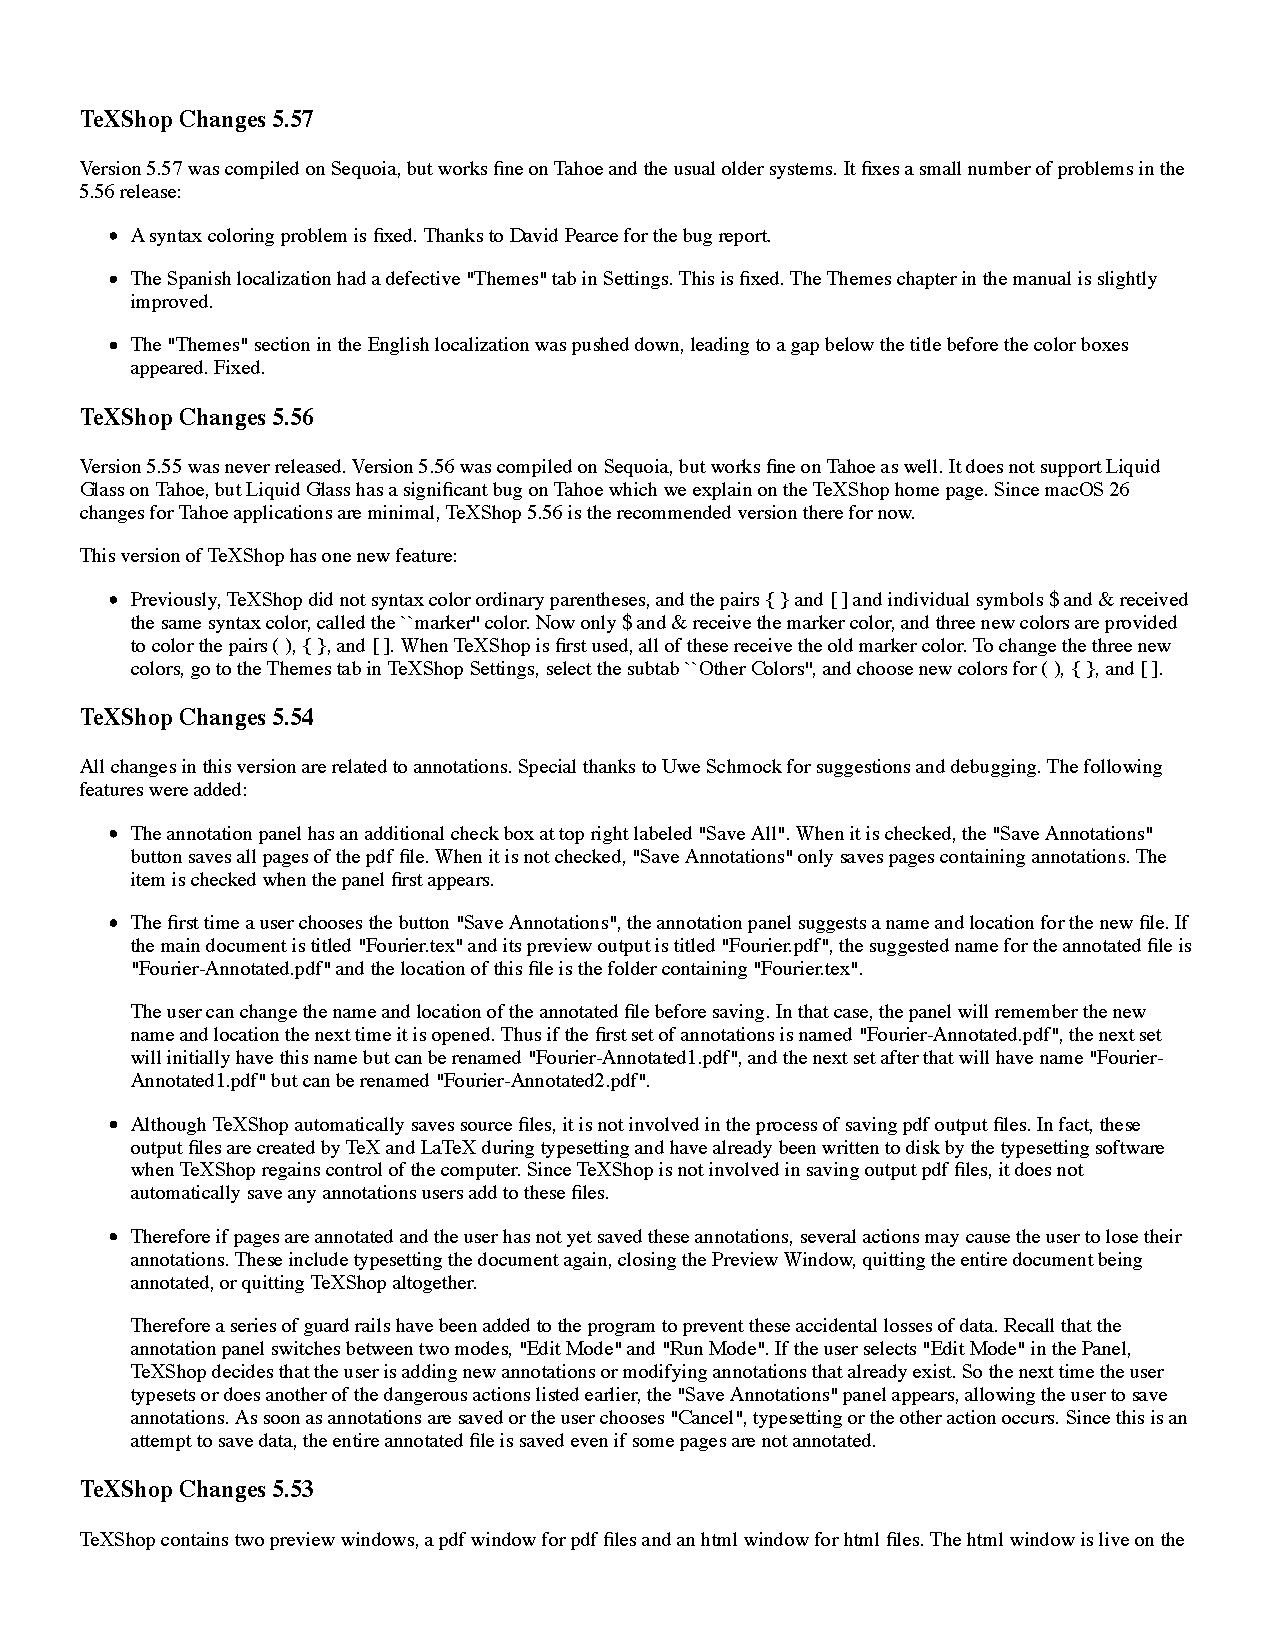
\includepdf[pages=-]{Changes-5.57.pdf}
\end{document}
